\begin{frame}{Input: Lattice Graph}
  \begin{definition}
    A \textbf{lattice graph} is a strongly connected directed
      multi-graph in which each edge $e$ is labeled with a rigid body
      transformation $T(e)$ and each $\edge{v}{T(e)}{w}$ has an
      inverse edge $\edge{w}{T(e)^{-1}}{v}$.  
    \end{definition}
    \begin{columns}[T] % align columns
      \begin{column}{.45\textwidth}
        \begin{figure}
  \centering
  \begin{tikzpicture}[->,>=stealth',shorten >=5pt,auto,node distance=1cm]
    \tikzstyle{every state}=[fill=blue,draw=none, text=white]
    \node[state, scale=0.7] (A)         {$0$};
    \path (A) edge [loop above] node {\footnotesize{Tr(0, 40)}} (A)
    edge [loop left]  node {\footnotesize{Tr(-40,0)}} (A)
    edge [loop below] node {\footnotesize{Tr(0, -40)}} (A)
    edge [loop right] node {\footnotesize{Tr(40, 0)}} (A);
  \end{tikzpicture}
\end{figure}
      \end{column}%
      \begin{column}{.45\textwidth}
        \begin{figure}
          \centering
          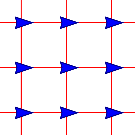
\includegraphics[scale=1]{figs/squarelattice}
        \end{figure}
      \end{column}%
    \end{columns}
\end{frame}